\setcounter{chapter}{8}
\chapter{Derivadas y aplicaciones}

\begin{theorybox}{Trazabilidad del capitulo piloto}
Este capitulo desarrolla las tipologias mapeadas en la matriz de cobertura como
\texttt{C09.S03} y \texttt{C09.S04}. La referencia de origen es
\texttt{sources/Relacion ejercicios tema 9. Derivadas y sus aplicaciones.pdf}, en concreto
los ejercicios de tangente en un punto y de tangente con pendiente dada o paralela a una
recta.
\end{theorybox}

\section{[C09.S03] Recta tangente y recta normal en un punto}

\subsection*{Objetivos de aprendizaje}
\begin{itemize}
  \item Interpretar la derivada en un punto como pendiente de la recta tangente.
  \item Escribir la ecuacion de la tangente y de la normal usando un punto de la curva.
  \item Reconocer el caso especial en el que la tangente es horizontal y la normal es vertical.
\end{itemize}

\subsection*{Prerrequisitos}
\begin{itemize}
  \item Reglas basicas de derivacion.
  \item Sustitucion de un valor en una funcion.
  \item Ecuacion de una recta en forma punto-pendiente.
\end{itemize}

\begin{theorybox}{Idea minima que hace falta}
Si una funcion \(f\) es derivable en \(x=a\), la pendiente de la recta tangente en ese punto es
\(f'(a)\). Si llamamos \(P(a,f(a))\) al punto de tangencia, entonces:
\[
  \text{tangente:}\quad y-f(a)=f'(a)(x-a).
\]
Si \(f'(a)\neq 0\), la recta normal es perpendicular a la tangente y su pendiente es
\(-1/f'(a)\):
\[
  \text{normal:}\quad y-f(a)=-\frac{1}{f'(a)}(x-a).
\]
Si \(f'(a)=0\), la tangente es horizontal y la normal es la recta vertical \(x=a\).
\end{theorybox}

\begin{methodbox}{Como reconocer este tipo de ejercicio y resolverlo}
\begin{enumerate}
  \item Busca la abscisa \(a\) o el punto donde se pide la tangente.
  \item Calcula \(f(a)\) para localizar el punto exacto de la curva.
  \item Deriva y obtiene la pendiente \(m_t=f'(a)\).
  \item Escribe la tangente con la forma \(y-f(a)=m_t(x-a)\).
  \item Para la normal:
  \begin{itemize}
    \item si \(m_t\neq 0\), usa \(m_n=-1/m_t\);
    \item si \(m_t=0\), escribe directamente \(x=a\).
  \end{itemize}
  \item Comprueba que la recta pasa por el punto calculado.
\end{enumerate}
\end{methodbox}

\begin{center}
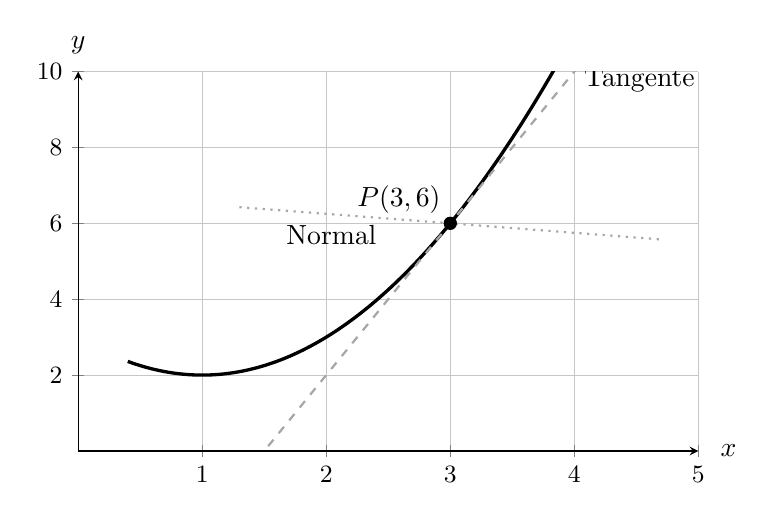
\begin{tikzpicture}
\begin{axis}[
  width=0.78\textwidth,
  height=6.4cm,
  axis lines=middle,
  xmin=0,
  xmax=5,
  ymin=0,
  ymax=10,
  samples=150,
  xlabel={$x$},
  ylabel={$y$},
  every axis x label/.style={at={(ticklabel* cs:1.02)},anchor=west},
  every axis y label/.style={at={(ticklabel* cs:1.02)},anchor=south},
  ticklabel style={font=\small},
  grid=both,
  grid style={line width=0.1pt, draw=gray!25},
  major grid style={line width=0.2pt, draw=gray!45},
]
\addplot[very thick, black, domain=0.4:4.6] {x^2 - 2*x + 3};
\addplot[thick, dashed, gray!70, domain=0.6:4.4] {4*x - 6};
\addplot[thick, dotted, gray!70, domain=1.3:4.7] {-x/4 + 27/4};
\addplot[only marks, mark=*, mark size=2.2pt] coordinates {(3,6)};
\node[anchor=south east] at (axis cs:3,6) {$P(3,6)$};
\node[anchor=south west] at (axis cs:4.0,9.2) {Tangente};
\node[anchor=north west] at (axis cs:1.6,6.2) {Normal};
\end{axis}
\end{tikzpicture}
\end{center}

\begin{solvedexample}{[EX-C09.S03-01] Tangente y normal a una parabola en un punto}
Calcula las ecuaciones de la recta tangente y de la recta normal a
\[
f(x)=x^2-2x+3
\]
en el punto de abscisa \(x=3\).

\textbf{Lectura del enunciado.} Nos dan la funcion y la abscisa del punto. Por tanto, primero
hay que localizar el punto de la grafica y despues hallar la pendiente de la tangente.

\textbf{Metodo elegido.} Usaremos derivada en un punto y la ecuacion punto-pendiente.

\textbf{Desarrollo.}
\[
f(3)=3^2-2\cdot 3+3=6.
\]
El punto de tangencia es \(P(3,6)\).

Derivamos:
\[
f'(x)=2x-2.
\]
La pendiente de la tangente en \(x=3\) es
\[
f'(3)=2\cdot 3-2=4.
\]
Entonces la tangente cumple
\[
y-6=4(x-3),
\]
y queda
\[
y=4x-6.
\]

La pendiente de la normal es la opuesta reciproca:
\[
m_n=-\frac{1}{4}.
\]
Su ecuacion es
\[
y-6=-\frac{1}{4}(x-3),
\]
es decir,
\[
y=-\frac{x}{4}+\frac{27}{4}.
\]

\textbf{Comprobacion.} Las dos rectas pasan por \(P(3,6)\). Ademas,
\[
4\cdot\left(-\frac{1}{4}\right)=-1,
\]
luego son perpendiculares.

\textbf{Respuesta final.}
\[
\boxed{y=4x-6}
\qquad\text{y}\qquad
\boxed{y=-\frac{x}{4}+\frac{27}{4}}.
\]
\end{solvedexample}

\begin{commonerror}{Cambiar solo el signo de la pendiente}
Si la tangente tiene pendiente \(4\), la normal no tiene pendiente \(-4\). Para obtener una
recta perpendicular en el plano hay que usar la opuesta reciproca, es decir, \(-1/4\). El
caso \(m_n=-4\) produciria una recta decreciente, pero no perpendicular a la tangente.
\end{commonerror}

\begin{guidedexercise}{[GX-C09.S03-01] Punto con pendiente negativa}
Halla la tangente y la normal a \(f(x)=x^2+1\) en \(x=-1\).

\textbf{Pista 1.} Empieza calculando el punto de la curva.

\textbf{Pista 2.} La derivada es \(f'(x)=2x\).
\end{guidedexercise}

\begin{shortanswer}{[GX-C09.S03-01]}
Tangente: \(y=-2x\). Normal: \(y=\dfrac{x}{2}+\dfrac{5}{2}\).
\end{shortanswer}

\begin{fullsolution}{[GX-C09.S03-01]}
El punto es \(P(-1,2)\), porque \(f(-1)=(-1)^2+1=2\). La pendiente de la tangente es
\(f'(-1)=2(-1)=-2\). Por tanto:
\[
y-2=-2(x+1)\quad\Longrightarrow\quad y=-2x.
\]
La pendiente de la normal es \(1/2\), luego:
\[
y-2=\frac{1}{2}(x+1)\quad\Longrightarrow\quad y=\frac{x}{2}+\frac{5}{2}.
\]
\end{fullsolution}

\begin{guidedexercise}{[GX-C09.S03-02] Tangente horizontal y normal vertical}
Estudia la tangente y la normal a \(f(x)=x^3-3x\) en \(x=1\).

\textbf{Pista 1.} Comprueba si la derivada vale cero.

\textbf{Pista 2.} Si la tangente es horizontal, la normal es vertical.
\end{guidedexercise}

\begin{shortanswer}{[GX-C09.S03-02]}
Tangente: \(y=-2\). Normal: \(x=1\).
\end{shortanswer}

\begin{fullsolution}{[GX-C09.S03-02]}
Se tiene \(f(1)=1-3=-2\), asi que el punto es \(P(1,-2)\). La derivada es
\[
f'(x)=3x^2-3.
\]
Entonces
\[
f'(1)=3-3=0.
\]
La tangente es horizontal y pasa por \(P\), asi que su ecuacion es \(y=-2\). La normal es la
recta perpendicular a una horizontal que pasa por \(x=1\), es decir, \(x=1\).
\end{fullsolution}

\subsection*{Practica autonoma graduada}

\begin{exercise}{[PX-C09.S03-01] Calcula la tangente y la normal a \(f(x)=x^2+2x\) en \(x=2\).}
\end{exercise}

\begin{exercise}{[PX-C09.S03-02] Calcula la tangente y la normal a \(f(x)=\dfrac{x+1}{x-1}\) en \(x=3\).}
\end{exercise}

\begin{exercise}{[PX-C09.S03-03] Calcula la tangente y la normal a \(f(x)=\sqrt{x+1}\) en \(x=3\).}
\end{exercise}

\begin{exercise}{[PX-C09.S03-04] Calcula la tangente y la normal a \(f(x)=e^x\) en \(x=0\).}
\end{exercise}

\begin{exercise}{[PX-C09.S03-05] Calcula la tangente y la normal a \(f(x)=\ln x\) en \(x=1\).}
\end{exercise}

\begin{exercise}{[PX-C09.S03-06] Calcula la tangente y la normal a \(f(x)=x^3\) en \(x=0\).}
\end{exercise}

\begin{shortanswer}{C09.S03 practica autonoma}
\begin{enumerate}[label=\textbf{PX-C09.S03-\arabic*:}, leftmargin=*]
  \item Tangente: \(y=6x-4\). Normal: \(y=-\dfrac{x}{6}+\dfrac{25}{3}\).
  \item Tangente: \(y=-\dfrac{x}{2}+\dfrac{7}{2}\). Normal: \(y=2x-4\).
  \item Tangente: \(y=\dfrac{x}{4}+\dfrac{5}{4}\). Normal: \(y=-4x+14\).
  \item Tangente: \(y=x+1\). Normal: \(y=-x+1\).
  \item Tangente: \(y=x-1\). Normal: \(y=-x+1\).
  \item Tangente: \(y=0\). Normal: \(x=0\).
\end{enumerate}
\end{shortanswer}

\begin{fullsolution}{C09.S03 practica autonoma}
\begin{enumerate}[label=\textbf{PX-C09.S03-\arabic*:}, leftmargin=*]
  \item \(f(2)=8\) y \(f'(x)=2x+2\), luego \(f'(2)=6\). Tangente:
  \[
  y-8=6(x-2)\Longrightarrow y=6x-4.
  \]
  Normal:
  \[
  y-8=-\frac{1}{6}(x-2)\Longrightarrow y=-\frac{x}{6}+\frac{25}{3}.
  \]

  \item \(f(3)=2\). Derivando,
  \[
  f'(x)=\frac{(x-1)-(x+1)}{(x-1)^2}=-\frac{2}{(x-1)^2},
  \]
  y entonces \(f'(3)=-1/2\). Tangente:
  \[
  y-2=-\frac{1}{2}(x-3)\Longrightarrow y=-\frac{x}{2}+\frac{7}{2}.
  \]
  Normal:
  \[
  y-2=2(x-3)\Longrightarrow y=2x-4.
  \]

  \item \(f(3)=2\) y
  \[
  f'(x)=\frac{1}{2\sqrt{x+1}},
  \]
  asi que \(f'(3)=1/4\). Tangente:
  \[
  y-2=\frac{1}{4}(x-3)\Longrightarrow y=\frac{x}{4}+\frac{5}{4}.
  \]
  Normal:
  \[
  y-2=-4(x-3)\Longrightarrow y=-4x+14.
  \]

  \item En \(x=0\), \(f(0)=1\) y \(f'(0)=e^0=1\). Tangente: \(y-1=x\), es decir, \(y=x+1\).
  Normal: \(y-1=-x\), luego \(y=-x+1\).

  \item En \(x=1\), \(f(1)=0\) y \(f'(1)=1\). Tangente: \(y=x-1\). Normal: \(y=-x+1\).

  \item \(f(0)=0\) y \(f'(x)=3x^2\), de modo que \(f'(0)=0\). La tangente es \(y=0\) y la
  normal es \(x=0\).
\end{enumerate}
\end{fullsolution}

\section{[C09.S04] Tangente con pendiente dada o paralela a una recta}

\subsection*{Objetivos de aprendizaje}
\begin{itemize}
  \item Traducir una condicion de paralelismo o pendiente a la ecuacion \(f'(x)=m\).
  \item Detectar si hay cero, una o varias tangentes que cumplen la condicion.
  \item Resolver casos con parametros antes de escribir la recta final.
\end{itemize}

\subsection*{Prerrequisitos}
\begin{itemize}
  \item Saber hallar la pendiente de una recta dada.
  \item Manejar la derivada como pendiente instantanea.
  \item Escribir la tangente en forma punto-pendiente.
\end{itemize}

\begin{theorybox}{Que cambia cuando la pendiente viene impuesta}
Si la tangente debe ser paralela a una recta \(y=mx+n\), su pendiente tiene que ser \(m\). El
problema se reduce a buscar los puntos de la curva donde
\[
f'(x)=m.
\]
Cada solucion \(x=a\) produce un posible punto de tangencia \(P(a,f(a))\). Despues solo hay
que escribir
\[
y-f(a)=m(x-a).
\]
Si aparece un parametro, primero se determina para que la condicion sobre la derivada sea
cierta.
\end{theorybox}

\begin{methodbox}{Como reconocer este tipo de ejercicio y resolverlo}
\begin{enumerate}
  \item Extrae la pendiente \(m\) de la condicion: ``pendiente dada'', ``paralela a'' o
  ``horizontal''.
  \item Resuelve la ecuacion \(f'(x)=m\).
  \item Calcula el punto o los puntos de tangencia sustituyendo en la funcion.
  \item Escribe una tangente por cada punto obtenido.
  \item Si hay parametros, resuelvelos antes de sustituir en la recta.
\end{enumerate}
\end{methodbox}

\begin{solvedexample}{[EX-C09.S04-01] Dos tangentes paralelas a una misma recta}
Halla las rectas tangentes a
\[
f(x)=x^3-3x+1
\]
que sean paralelas a la recta \(y=9x-4\).

\textbf{Lectura del enunciado.} Ser paralela a \(y=9x-4\) significa tener pendiente \(9\).

\textbf{Metodo elegido.} Igualamos la derivada a \(9\).

\textbf{Desarrollo.}
\[
f'(x)=3x^2-3.
\]
Imponemos la pendiente:
\[
3x^2-3=9 \Longrightarrow 3x^2=12 \Longrightarrow x^2=4.
\]
Por tanto, hay dos abscisas:
\[
x=-2 \qquad\text{y}\qquad x=2.
\]

Calculamos los puntos:
\[
f(-2)=(-2)^3-3(-2)+1=-1,
\qquad
f(2)=2^3-3\cdot 2+1=3.
\]
Luego los puntos de tangencia son \((-2,-1)\) y \((2,3)\).

La tangente en \((-2,-1)\) es
\[
y+1=9(x+2)\Longrightarrow y=9x+17.
\]
La tangente en \((2,3)\) es
\[
y-3=9(x-2)\Longrightarrow y=9x-15.
\]

\textbf{Comprobacion.} Las dos rectas tienen pendiente \(9\), luego son paralelas a la recta
dada. Ademas, cada una pasa por su punto de tangencia.

\textbf{Respuesta final.}
\[
\boxed{y=9x+17}
\qquad\text{y}\qquad
\boxed{y=9x-15}.
\]
\end{solvedexample}

\begin{commonerror}{Olvidar que puede haber mas de una tangente}
Resolver \(f'(x)=m\) no siempre da una unica abscisa. En funciones no lineales es habitual que
aparezcan dos o mas puntos con la misma pendiente. Si se escribe una sola tangente sin revisar
todas las soluciones de la ecuacion, la respuesta queda incompleta.
\end{commonerror}

\begin{guidedexercise}{[GX-C09.S04-01] Pendiente dada}
Escribe la ecuacion de la tangente a \(f(x)=x^2-4x\) que tenga pendiente \(2\).

\textbf{Pista 1.} La condicion principal es \(f'(x)=2\).

\textbf{Pista 2.} Una vez hallada la abscisa, calcula el punto de tangencia.
\end{guidedexercise}

\begin{shortanswer}{[GX-C09.S04-01]}
\(y=2x-9\).
\end{shortanswer}

\begin{fullsolution}{[GX-C09.S04-01]}
Derivamos:
\[
f'(x)=2x-4.
\]
Imponemos la pendiente \(2\):
\[
2x-4=2 \Longrightarrow x=3.
\]
El punto de tangencia es
\[
f(3)=9-12=-3.
\]
Por tanto,
\[
y+3=2(x-3)\Longrightarrow y=2x-9.
\]
\end{fullsolution}

\begin{guidedexercise}{[GX-C09.S04-02] Paralelismo con una recta}
Halla la tangente a \(f(x)=\sqrt{x+4}\) que sea paralela a la recta
\[
y=\frac{1}{4}x-2.
\]

\textbf{Pista 1.} La pendiente buscada es \(1/4\).

\textbf{Pista 2.} Resuelve \(\dfrac{1}{2\sqrt{x+4}}=\dfrac{1}{4}\).
\end{guidedexercise}

\begin{shortanswer}{[GX-C09.S04-02]}
\(y=\dfrac{x}{4}+2\).
\end{shortanswer}

\begin{fullsolution}{[GX-C09.S04-02]}
La derivada es
\[
f'(x)=\frac{1}{2\sqrt{x+4}}.
\]
Imponemos la pendiente \(1/4\):
\[
\frac{1}{2\sqrt{x+4}}=\frac{1}{4}
\Longrightarrow 4=2\sqrt{x+4}
\Longrightarrow \sqrt{x+4}=2
\Longrightarrow x=0.
\]
El punto correspondiente es \(P(0,2)\). Luego la tangente es
\[
y-2=\frac{1}{4}(x-0),
\]
es decir,
\[
y=\frac{x}{4}+2.
\]
\end{fullsolution}

\subsection*{Practica autonoma graduada}

\begin{exercise}{[PX-C09.S04-01] Halla la tangente a \(f(x)=x^2+1\) con pendiente \(4\).}
\end{exercise}

\begin{exercise}{[PX-C09.S04-02] Halla las tangentes a \(f(x)=x^3\) paralelas a la recta \(y=12x+1\).}
\end{exercise}

\begin{exercise}{[PX-C09.S04-03] Halla la tangente a \(f(x)=\ln x\) paralela a la recta \(y=x+3\).}
\end{exercise}

\begin{exercise}{[PX-C09.S04-04] Halla la tangente a \(f(x)=e^x\) cuya pendiente sea \(e^2\).}
\end{exercise}

\begin{exercise}{[PX-C09.S04-05] Halla las tangentes horizontales de \(f(x)=x+\dfrac{1}{x}\).}
\end{exercise}

\begin{exercise}{[PX-C09.S04-06] Sea \(f(x)=x^2+ax\). Determina \(a\) para que la tangente en
\(x=1\) sea paralela a la recta \(y=5x-2\), y escribe despues esa tangente.}
\end{exercise}

\begin{shortanswer}{C09.S04 practica autonoma}
\begin{enumerate}[label=\textbf{PX-C09.S04-\arabic*:}, leftmargin=*]
  \item \(y=4x-3\).
  \item \(y=12x+16\) y \(y=12x-16\).
  \item \(y=x-1\).
  \item \(y=e^2x-e^2\).
  \item \(y=2\) y \(y=-2\).
  \item \(a=3\) y la tangente es \(y=5x-1\).
\end{enumerate}
\end{shortanswer}

\begin{fullsolution}{C09.S04 practica autonoma}
\begin{enumerate}[label=\textbf{PX-C09.S04-\arabic*:}, leftmargin=*]
  \item \(f'(x)=2x\). Imponiendo \(2x=4\) se obtiene \(x=2\). Como \(f(2)=5\),
  \[
  y-5=4(x-2)\Longrightarrow y=4x-3.
  \]

  \item \(f'(x)=3x^2\). Imponemos \(3x^2=12\), luego \(x=\pm 2\). Los puntos son
  \((2,8)\) y \((-2,-8)\). Las tangentes:
  \[
  y-8=12(x-2)\Longrightarrow y=12x-16,
  \]
  \[
  y+8=12(x+2)\Longrightarrow y=12x+16.
  \]

  \item \(f'(x)=1/x\). Igualando a \(1\), resulta \(x=1\). Como \(f(1)=0\),
  \[
  y=x-1.
  \]

  \item En una exponencial, \(f'(x)=e^x\). Si la pendiente debe ser \(e^2\), entonces
  \(e^x=e^2\) y \(x=2\). El punto es \((2,e^2)\), asi que
  \[
  y-e^2=e^2(x-2)\Longrightarrow y=e^2x-e^2.
  \]

  \item
  \[
  f'(x)=1-\frac{1}{x^2}.
  \]
  Las tangentes horizontales cumplen \(f'(x)=0\):
  \[
  1-\frac{1}{x^2}=0 \Longrightarrow x^2=1 \Longrightarrow x=\pm 1.
  \]
  En \(x=1\), \(f(1)=2\), luego la tangente es \(y=2\). En \(x=-1\), \(f(-1)=-2\), luego la
  tangente es \(y=-2\).

  \item Derivamos:
  \[
  f'(x)=2x+a.
  \]
  En \(x=1\) debe valer \(5\):
  \[
  2+a=5 \Longrightarrow a=3.
  \]
  Entonces \(f(1)=1+3=4\). La tangente pedida es
  \[
  y-4=5(x-1)\Longrightarrow y=5x-1.
  \]
\end{enumerate}
\end{fullsolution}

\begin{challenge}{[CH-C09-01] Transferencia a una situacion nueva}
La altura de una pelota, en metros, viene dada por
\[
h(t)=-t^2+6t+5,
\]
donde \(t\) se mide en segundos.

\begin{enumerate}
  \item Determina el instante en el que la tangente a la grafica es horizontal.
  \item Escribe la ecuacion de esa tangente.
  \item Interpreta el resultado en el contexto del problema.
\end{enumerate}
\end{challenge}

\begin{shortanswer}{[CH-C09-01]}
La tangente es horizontal en \(t=3\). Su ecuacion es \(y=14\). En ese instante la pelota
alcanza una altura maxima instantanea y la velocidad vertical es cero.
\end{shortanswer}

\begin{fullsolution}{[CH-C09-01]}
La tangente es horizontal cuando \(h'(t)=0\). Como
\[
h'(t)=-2t+6,
\]
se cumple
\[
-2t+6=0 \Longrightarrow t=3.
\]
La altura en ese instante es
\[
h(3)=-9+18+5=14.
\]
Por tanto, la tangente en ese punto es la recta horizontal \(y=14\). En contexto, significa
que la pelota se encuentra en un punto alto de su trayectoria y en ese instante su velocidad
vertical es nula.
\end{fullsolution}

\begin{selfcheck}
\begin{itemize}
  \item Distingo entre ``tangente en un punto'' y ``tangente con pendiente impuesta''.
  \item Recuerdo que la normal usa la opuesta reciproca, salvo cuando la tangente es horizontal.
  \item Reviso siempre si la ecuacion \(f'(x)=m\) tiene una o varias soluciones.
  \item Compruebo que cada recta final pasa por su punto de tangencia.
\end{itemize}
\end{selfcheck}

\begin{extension}{Puente a ejercicios de ampliacion}
En la relacion del tema 9 aparecen, ademas, ejercicios de estudio global, derivabilidad a
trozos y optimizacion. Quedan ya mapeados en \texttt{data/coverage\_matrix.csv} como
\texttt{C09.S05}, \texttt{C09.S06}, \texttt{C09.S07} y \texttt{C09.S08}, listos para la
siguiente fase de redaccion.
\end{extension}
